\documentclass[11pt]{article}
% Set margins to 0pt to prevent unnecessary page overflows
\usepackage[paperwidth=2550px, paperheight=3300px, margin=0pt]{geometry}
\usepackage{tikz}
\usepackage{xcolor}
\usepackage{hyperref}

% Define color palette for Levels 1–5
\definecolor{level1bg}{RGB}{213, 176, 241} % Light Purple
\definecolor{level2bg}{RGB}{213, 128, 241} % Purple
\definecolor{level3bg}{RGB}{136, 232, 159} % Green
\definecolor{level4bg}{RGB}{115, 151, 226} % Blue
\definecolor{level5bg}{RGB}{200, 200, 200} % Gray

\definecolor{accentgold}{RGB}{185, 142, 50}
\definecolor{navytext}{RGB}{20, 30, 75}
\definecolor{bordergray}{RGB}{200, 200, 200}

\pagestyle{empty}
\parindent=0pt

% Badge Dimensions @ 300 DPI: 2.25 in x 3.375 in -> 675px x 1012.5px
\newcommand{\badge}[3]{%
  \begin{scope}
    % Outer border / cutting guideline
    \draw[bordergray, line width=1.5px] (0, 0) rectangle (675px, 1012.5px);

    % Top Access Level Header Block
    \fill[#2] (0, 795px) rectangle (675px, 1012.5px);
    \fill[accentgold] (0, 786px) rectangle (675px, 795px);

    % Access Level Text Field
    \node[anchor=center] at (337.5px, 903px) {%
      \TextField[
        name=AccessLevel-#1,
        width=630px,
        height=96px,
        bordercolor=,
        backgroundcolor=,
        default=#3,
        charsize=64pt,
        align=1
      ]{}%
    };

    % Central Photo Frame Border
    \draw[accentgold, line width=4.5px] (97.5px, 285px) rectangle (577.5px, 735px);

    % Interactive Photo Upload Button Field
    \node[anchor=center] at (337.5px, 510px) {%
      \PushButton[
        name=PhotoButton-#1,
        width=480px,
        height=450px,
        bordercolor=,
        backgroundcolor=,
        onclick={this.buttonImportIcon();}
      ]{Click to Select Photo}%
    };

    % Name / User Field
    \node[anchor=center] at (337.5px, 216px) {%
      \TextField[
        name=FullName-#1,
        width=600px,
        height=75px,
        bordercolor=,
        backgroundcolor=,
        charsize=48pt,
        default=Insert Name Here,
        align=1
      ]{}%
    };

    % Bottom Expiration Date Footer Block
    \fill[#2] (0, 0) rectangle (675px, 135px);

    % Expiration Date Field
    \node[anchor=east] at (645px, 67.5px) {%
      \TextField[
        name=ExpDate-#1,
        width=390px,
        height=60px,
        bordercolor=,
        backgroundcolor=,
        charsize=24pt,
        default=Exp: YYYY-MM-DD,
        align=2
      ]{}%
    };
  \end{scope}%
}

\begin{document}

\Form % Initialize interactive PDF Form environment

\nointerlineskip
\vbox to \paperheight{
  \vss
  \centering
  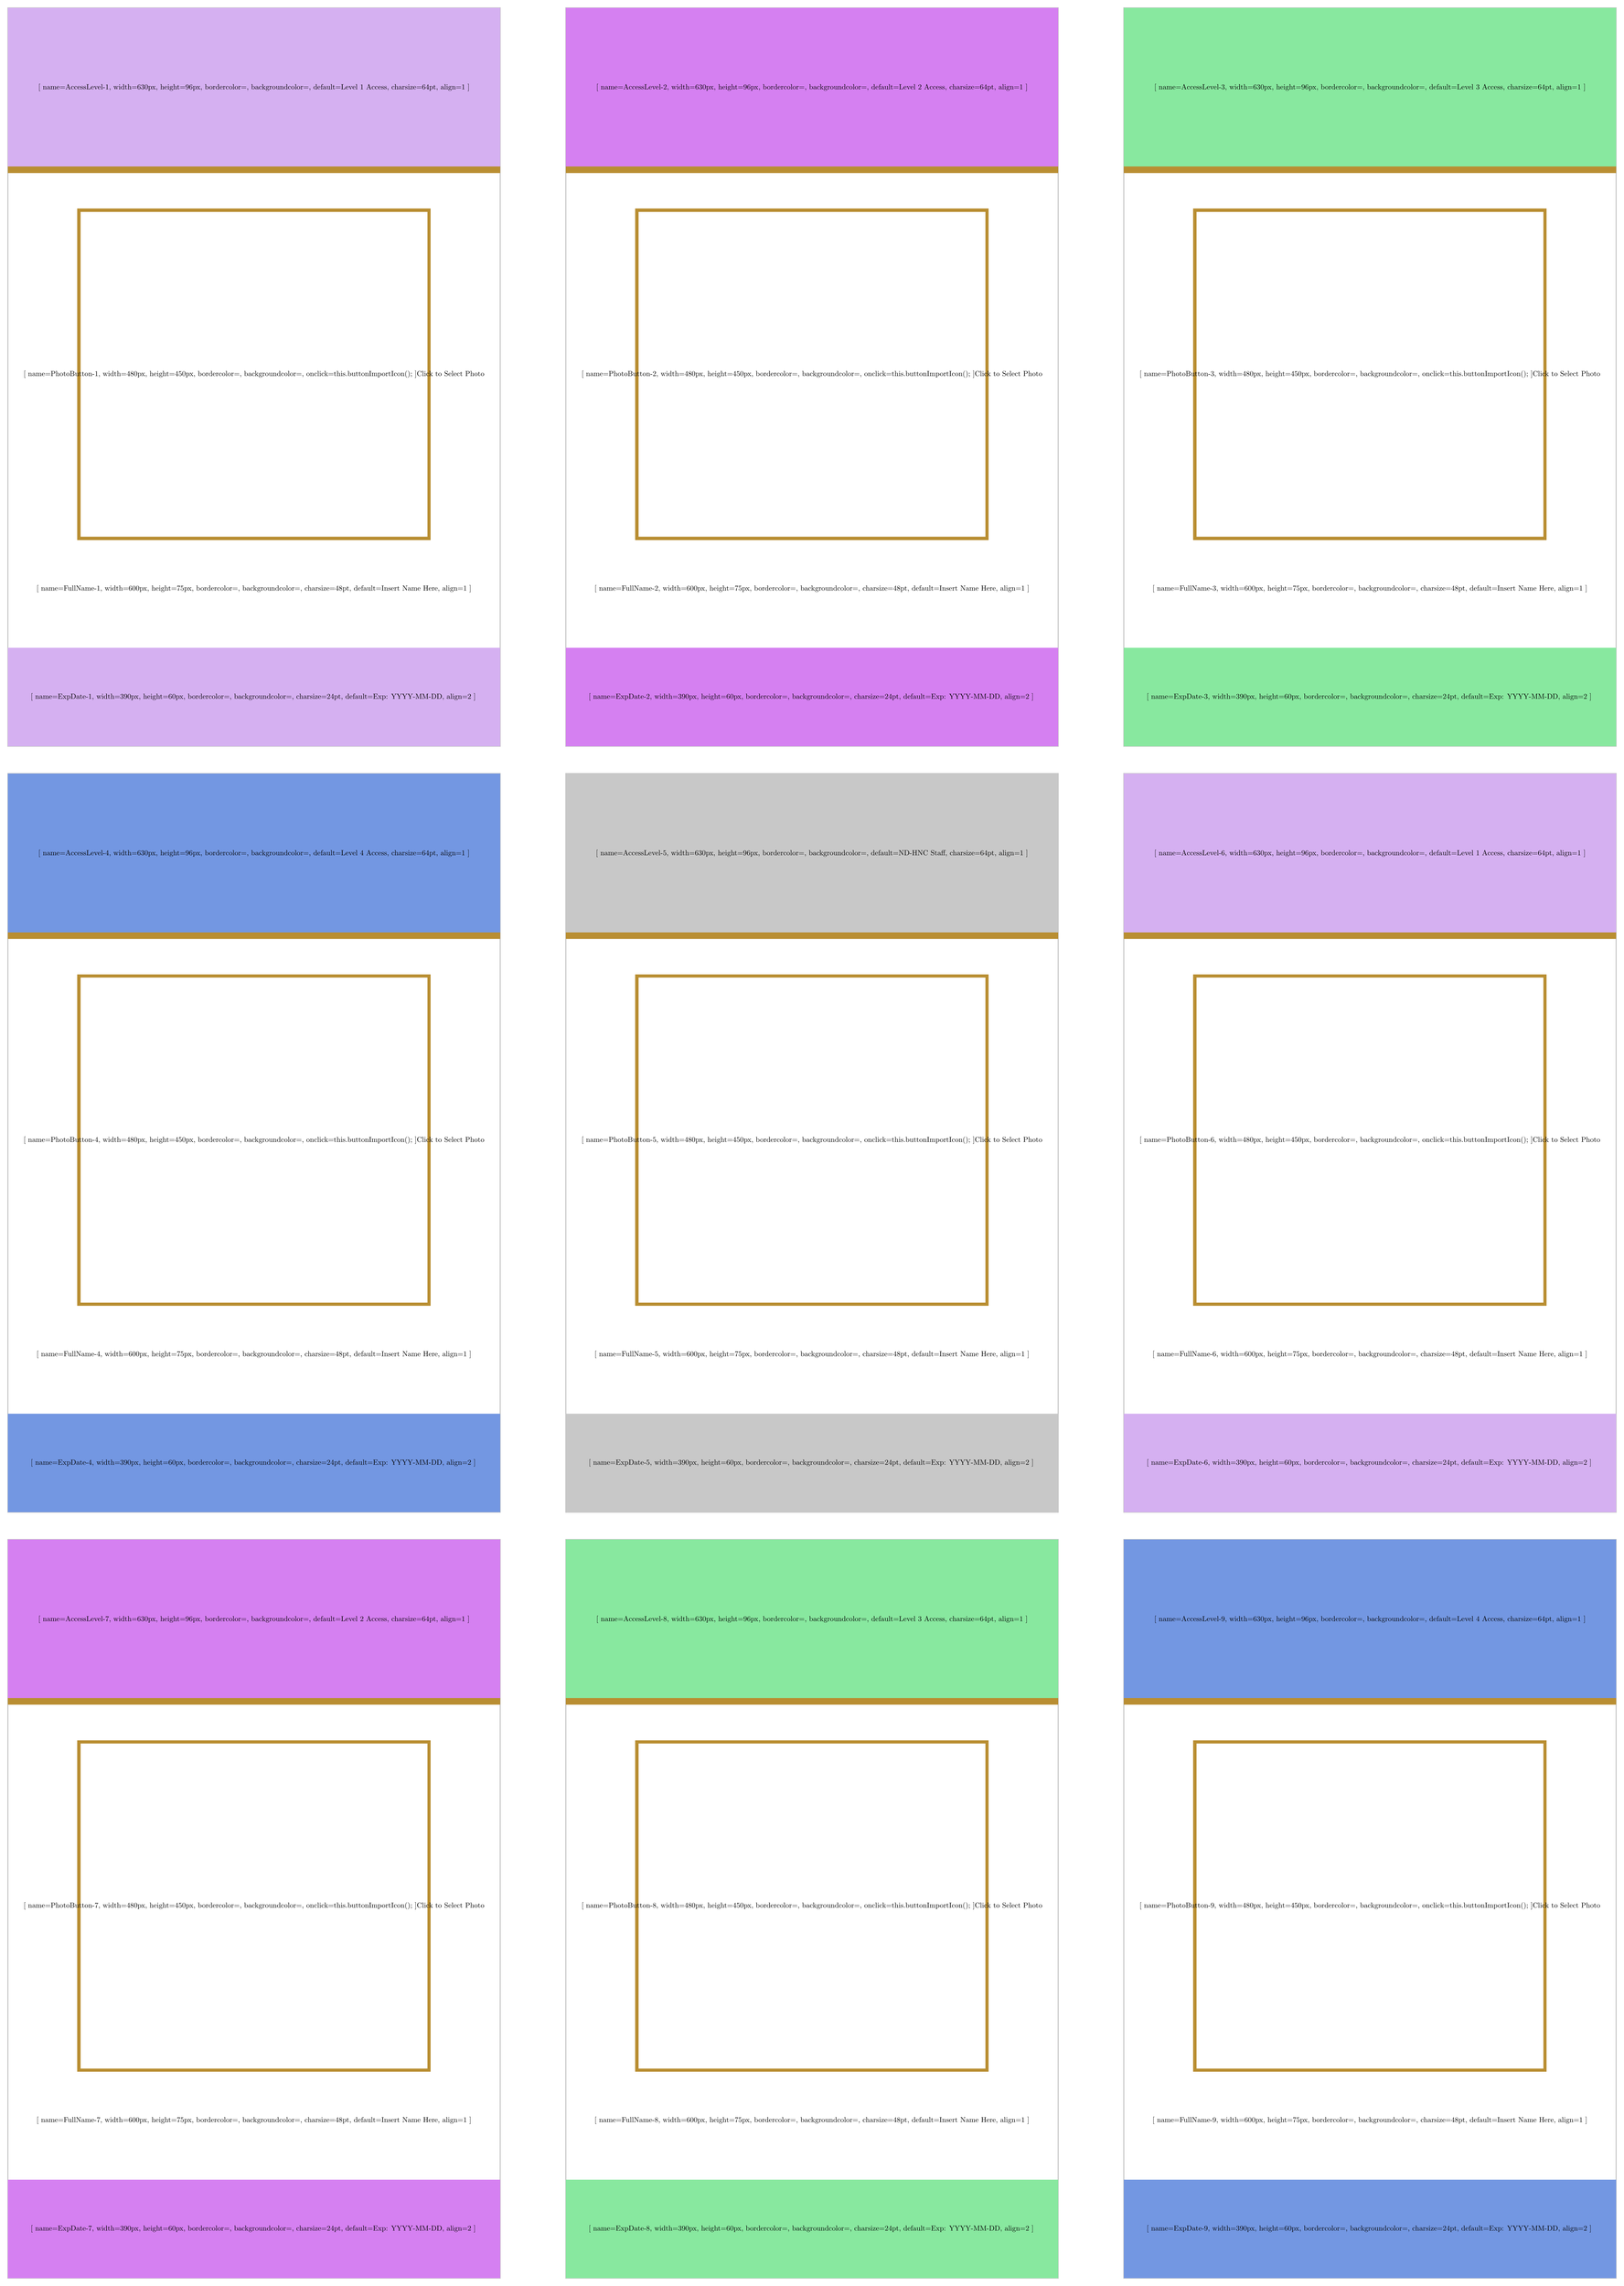
\begin{tikzpicture}[x=1px, y=1px]

    % Row 1 (Top)
    \begin{scope}[shift={(0px, 2100px)}]
      \badge{1}{level1bg}{Level 1 Access}
    \end{scope}
    \begin{scope}[shift={(765px, 2100px)}]
      \badge{2}{level2bg}{Level 2 Access}
    \end{scope}
    \begin{scope}[shift={(1530px, 2100px)}]
      \badge{3}{level3bg}{Level 3 Access}
    \end{scope}

    % Row 2 (Middle)
    \begin{scope}[shift={(0px, 1050px)}]
      \badge{4}{level4bg}{Level 4 Access}
    \end{scope}
    \begin{scope}[shift={(765px, 1050px)}]
      \badge{5}{level5bg}{ND-HNC Staff}
    \end{scope}
    \begin{scope}[shift={(1530px, 1050px)}]
      \badge{6}{level1bg}{Level 1 Access}
    \end{scope}

    % Row 3 (Bottom)
    \begin{scope}[shift={(0px, 0px)}]
      \badge{7}{level2bg}{Level 2 Access}
    \end{scope}
    \begin{scope}[shift={(765px, 0px)}]
      \badge{8}{level3bg}{Level 3 Access}
    \end{scope}
    \begin{scope}[shift={(1530px, 0px)}]
      \badge{9}{level4bg}{Level 4 Access}
    \end{scope}

  \end{tikzpicture}
  \vss
}

\end{document}